% !TeX root=../../../main.tex
\chapter{مروری بر کار‌های پیشین}
%\thispagestyle{empty} 
توضیح خطا
\lf{Fault Explanation}
و
متمرکز کردن خطا
\lf{Fault Localization}
روش‌هایی هستند
که فرآیند رفع‌ایراد نرم‌افزار را تسهیل می‌کنند.
توضیح‌خطا روش‌هایی را شامل می‌شود که به کاربر کمک می‌کند که با استفاده از یک مثال‌نقض یا یک دنباله از اجرای سیستم به ماهیت خطا و در نتیجه روش اصلاح خطا پی ببرد.
در روش‌های متمرکز کردن خطا هدف مشخص کردن بخشی از سیستم است که عامل خطا بوده و امکان اندازه‌گیری کمی و مقایسه آن با دیگر بخش‌ها وجود دارد
\cite{groce2006error}.
یکی از روش‌های توضیح خطا پیدا کردن علت خطا بر اساس استدلال مبتنی بر خلاف واقع که توسط لوئیس در
\cite{lewis1973counterfactuals}
ارائه شده می‌باشد که در پژوهش‌هایی مانند
\cite{zeller2009programs,groce2006error,groce2003went}
استفاده شده است.
هالپرن و پرل در
\cite{hp}
تعریفی مبتنی بر استدلال خلاف واقع لوئیس ارائه کردند که توانسته است برخی از مشکلات تعریف لوئیس در پیدا کردن علت در سناریو‌های پیچیده را بر طرف کند.
در ادامه برخی از پژوهش‌هایی که از تعریف هالپرن و پرل برای توضیح خطا استفاده کرده‌اند را مورد بررسی قرار می‌دهیم.

\section{تخمین پوشش}
در
\cite{Chockler_Halpern_Kupferman_2008}
نویسندگان از مدل
HP
برای تخمین میزان پوشش
\lf{Covering}
سیستم توسط یک توصیف در فرآیند وارسی مدل استفاده کرده‌اند.
معیارهای پوشش معمولا در فرآیند تست سیستم استفاده می‌شوند و مشخص کننده‌ درصدی از اجزا یا حالت‌های سیستم هستند که توسط مجموعه‌ی تست‌ها مورد استفاده یا بازدید قرار می‌گیرند.
در فرآیند وارسی مدل همه‌ی حالت‌های سیستم بررسی می‌شوند به همین دلیل در این شرایط اگر تغییر یک حالت منجر به نقض ویژگی توصیف شده شود این حالت پوشش داده شده توسط ویژگی تعریف می‌شود.
با استفاده از مفهوم مسئولیت
\lf{Responsiblity}
که در
\cite{hp2}
تعریف شده است، نویسندگان این پژوهش به جای در نظر گرفتن مقدار ۰ و ۱ برای پوشیده شدن یا نشدن از درجه‌ی مسئولیت استفاده می‌کنند.
همانطور که مشخص است این پژوهش به اصلاح و بهبود توصیف ویژگی کمک می‌کند و نه پیدا کردن علت خطا.
در این پژوهش همانند پژوهش جاری به شکل مستقیم از تعریف 
HP
استفاده شده است.

\section{علت خطا در مثال نقض}
در
\cite{chockler}
نویسندگان سیستم را به صورت یک سیستم انتقال
\lf{Transition System}
در نظر می‌گیرند که در آن هر حالت یک نگاشت از یک مجموعه‌ی متغیر‌های بولی به مقادیر درست و غلط است.
در این پژوهش با استفاده از تعریف علت واقعی در یک مثال نقض یک ویژگی توصیف شده در
LTL
\lf{Linear Temporal Logic}
یک دوتایی‌ متغیر و حالت به عنوان علت واقعی در نظر گرفته می‌شود.
در همین پژوهش یک الگوریتم تقریبی برای پیدا کردن همه‌ی علت‌ها در یک مثال نقض داده شده ارائه شده است و ابزاری برای نمایش این علت‌ها به صورت گرافیکی به کاربر توسعه داده شده و در ابزار درستی‌سنجی
RuleBase PE
متعلق به
IBM
گنجانده شده است.
\begin{figure}
    \centering
    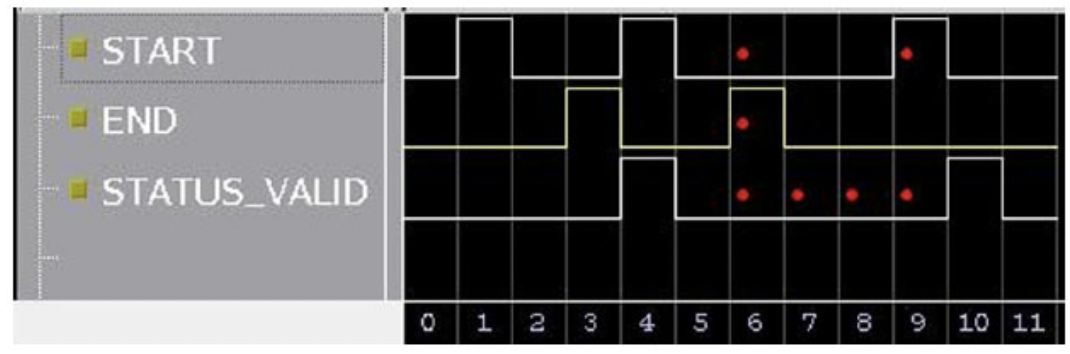
\includegraphics[width=15cm]{chockler.png}
    \caption{رابط کاربری ابزار
        RuleBase PE
    }
    \label{fig:rulebase}
\end{figure}
تصویر
\ref{fig:rulebase}
رابط کاربری ابزار 
RuleBase PE
را پس از پیدا کردن یک مثال نقض برای ویژگی زیر نشان می‌دهد:
\begin{align*}
    \boldsymbol{\mr{G}}((\neg \texttt{START} \wedge \neg \texttt{STATUS\_VALID} \wedge \texttt{END}) 
    \ra [\neg \texttt{START}\ \boldsymbol{\mr{U}}\ \texttt{STATUS\_VALID}])
\end{align*}
در این تصویر نقاط قرمز علت‌های واقعی هستند که با الگوریتم تقریبی پیاده‌سازی شده پیدا شده‌اند.
 این پژوهش یکی از کاربردی‌ترین استفاده‌ها از توضیح خطا و پیدا کردن علت خطا را نشان می‌دهد. 
در این پژوهش سعی شده است تا علت خطا در یک مثال نقض پیدا شود و به همین دلیل مقدار متغیر‌ها در حالت‌ها به عنوان علت پیدا می‌شوند در حالی که در پژوهش جاری هدف پیدا کردن علت خطا در کل سیستم است و در واقع ساختار‌های سیستم، مثلا وجود یا عدم وجود روابط تعارض یا فعال‌سازی به عنوان علت خطا پیدا می‌شوند.
اما همانند پژوهش جاری در این پژوهش هم به شکل مستقیم و بدون تغییر از تعریف 
HP
استفاده شده است.

\section{چک کردن علیت}
در پژوهش 
\cite{causality-checking}
نویسندگان تعریفی از علت‌ واقعی که الهام گرفته از تعریف 
HP
است ارائه می‌کنند و الگوریتم آن‌ها بر اساس این تعریف در حین اجرای فرآیند وارسی مدل
\lf{Model Checking}
علت‌ها را پیدا کرده و در نتیجه در انتهای وارسی مدل اگر سیستم ویژگی مورد نظر را نقض کرد به جای برگرداندن یک مثال نقض، رویداد‌هایی که علت رخداد خطا بوده‌اند را بر می‌گرداند.
در این پژوهش یک منطق برای توصیف یک دنباله از رویداد عملیات‌های سیستم ارائه شده است و فرمول‌های این منطق به عنوان علت خطا در نظر گرفته می‌شوند. 
این پژوهش هم همانند
\cite{chockler}
سعی بر پیدا کردن همه‌ی علت‌های بروز خطا دارد و علت‌ها عملا دنباله‌هایی از اجرای سیستم هستند. 
تفاوت اصلی این کار با پژوهش جاری در این است که در این پژوهش علت خطا در رفتارهای سیستم جستجو می‌شود در حالی که در پژوهش جاری علت خطا در میان عناصر ساختاری سیستم جستجو می‌شود.
این روش تنها برای ویژگی‌های دسترس‌پذیری ارائه شده است.
در
\cite{Caltais-LTL}
نویسندگان این روش‌ را برای ویژگی‌های دلخواه توصیف شده توسط
LTL
تعمیم دادند.

\section{علت واقعی در خودکاره‌های زمان‌دار}
در
\cite{kolbl2020dynamic}
نویسندگان از تعریف 
HP
برای پیدا کردن علت خطا در خودکاره‌های زمان‌دار
\lf{Timed Automata}
استفاده کرده‌اند.
در درستی‌سنجی خودکاره‌های زمان‌دار یک ابزار وارسی مدل بلا درنگ نقض ویژگی‌ را در قالب یک رد تشخیصی زمان‌دار 
\lf{Timed Diagnostic Trace}
که در واقع یک مثال‌نقض است بر می‌گرداند.
یک 
TDT
در واقع یک دنباله متناوب از انتقال تاخیر
\lf{Transition Delay}
و
انتقال عملیات
\lf{Delay Transition}
ها است که در آن مقدار تاخیر‌ها به صورت سمبلیک مشخص شده‌اند.
هدف این پژوهش پیدا کردن مقادیری یا دامنه‌ای از مقادیر برای این تاخیر‌های سمبلیک است که بروز خطا را اجتناب ناپذیر می‌کنند یا به عبارت دیگر علت واقعی هستند.
در این پژوهش اما به صورت مستقیم از تعریف 
HP
استفاده نشده است و بر اساس آن تعریفی برای علت واقعی نقض ویژگی در یک 
TDT
بیان شده است.

\section{چارچوب علیت بر اساس رد سیستم}
در 
\cite{gossler2013general}
نویسندگان این مساله را مطرح می‌کنند که تعریف ارائه شده توسط هالپرن و پرل ذاتا یک مدل بر اساس منطق گزاره‌ای
\lf{Propositional Logic}
است و به همین دلیل برای درستی‌سنجی پردازه‌ها ایده‌آل نیست.
در این پژوهش یک فرمالیسم و تعریف جدید برای علیت بر اساس تعریف 
HP
ارائه می‌شود که در آن از رد‌
\lf{Trace}
های سیستم به جای متغیر‌ها در مدل 
HP
استفاده می‌شود و امکان ترکیب
\lf{Composition}
چند مدل با یکدیگر را فراهم می‌کند.


\section{استدلال مبتنی بر علیت در 
HML
}
در
\cite{decomposing}
نویسندگان از مفهوم استدلال مبتنی در سیستم‌انتقال برچسب‌دار
\lf{Labeled Transition System}
و 
HML
\lf{Hennesy Milner Loigc} \cite{hml}
استفاده کرده‌اند.
در این پژوهش سیستم با استفاده از یک سیستم انتقال برچسب‌دار مدل می‌شود و رفتار ناامن توسط یک فرمول در قالب
HML
توصیف می‌شود.
سپس یک تعریف جدید که برگرفته شده از تعریف
HP
است با استفاده از این مدل‌ها برای علت واقعی بیان می‌شود.
در این تعریف از مفهومی به نام عدم‌وقوع
\lf{Non-Occurrence}
رویدادها که پیش‌تر در 
\cite{causality-checking}
مطرح شده بود استفاده می‌شود.
شهود کلی مفهوم عدم‌وقوع در علیت این است که در کنار اینکه رخ‌دادن برخی از رویداد‌ها منجر به خطا می‌شود، رخ ندادن رویداد‌ها هم می‌تواند به عنوان علت در نظر گرفته شود.
در تعریف ارائه شده در این پژوهش مجموعه‌ای از محاسبه‌
\lf{Computation}
های سیستم به عنوان علت برقراری یک فرمول 
HML
در سیستم که رفتار نا امن
\lf{Unsafe Behavior}
را توصیف می‌کند تعریف می‌شود.
هر محاسبه شامل یک دنباله از عملیات‌های سیستم در کنار تعدادی عملیات دیگر، که عدم وقوع آن‌ها هم جزئی از علت است، در نظر گرفته می‌شود.
به عبارت دیگر یک محاسبه را می‌توان شامل دو جز در نظر گرفت.
جز اول یک اجرای سیستم است که منجر به خطا می‌شود.
جز دوم مجموعه‌ای از اجراهای سیستم‌ است که منجر به خطا نمی‌شوند و حاصل جایگذاری
\lf{Interleaving}
برخی از عملیات‌ها در جز اول این محاسبه هستند.
عملیات‌های جایگذاری شده عملیات‌هایی هستند که عدم وقوع آن‌ها به عنوان علت بروز 
خطا در نظر گرفته می‌شود.
در این تعریف علت‌ واقعی به گونه‌ای تعریف شده است که محاسباتی‌ که منجر به فعال شدن فرمول 
HML
در سیستم می‌شوند به عنوان علت در نظر گرفته می‌شوند.
در این تعریف شروطی مشابه با شروط موجود در تعریف 
HP
در نظر گرفته شده است.
در 
\cite{causal-hml}
نویسندگان تعریف خود را بهبود دادند تا تطابق بیشتری با تعریف 
HP
داشته باشد.
علاوه بر این در این پژوهش ثابت شده است که این تعریف از علت در سیستم‌هایی که ارتباط همگام
\lf{Synchronized}
شده دارند قابل ترکیب نیست ولی در حالتی که سیستم‌ها ارتباط همگام نداشته باشند امکان ترکیب یا شکستن آن وجود دارد.
نتایج حاصل از این پژوهش یکی از انگیزه‌های اصلی پژوهش جاری بود برای اینکه با انتخاب یک مدل معنایی یا تعریف علیت متفاوت امکان ترکیب آن برای سیستم‌های همگام شده بررسی شود.
در ادامه به بررسی شباهت‌ها و تفاوت‌های این پژوهش و پژوهش جاری می‌پردازیم
اولا در این پژوهش تعریف جدیدی از علت واقعی ارائه شده است در حالی که در پژوهش جاری مستقیما از تعریف ارائه شده در
\cite{hp}
استفاده شده است.
در پژوهش جاری تمرکز بر پیدا کردن یک علت برای بروز خطا در سیستم است در حالی که در این پژوهش همه‌ی علل خطا مورد بررسی قرار می‌گیرند.
پژوهش جاری علل خطا را در ساختار‌های سیستم جستجو می‌کند در حالی که این پژوهش در میان رفتار‌های سیستم به دنبال علل خطا می گردد.

\section{جمع‌بندی}
همان طور که بررسی شد پژوهش‌های متعددی در زمینه‌ی توضیح خطا ارائه شده است که نشان از اهمیت این مساله در فرآیند درستی‌سنجی و اشکال‌زدایی دارد.
همچنین تعریف 
HP
هم مورد توجه زیادی برای پیدا کردن علت خطا قرار گرفته است.
یکی از مهم‌ترین تمایز‌های پژوهش جاری با پژوهش‌های پیشین در المان‌هایی است که در آن علت خطا پیدا می‌شود. 
همانطور که بررسی شد در تمامی پژوهش‌های پیشین در این زمینه علت خطا در میان رفتارهای سیستم جستجو می‌شود. 
اما در پژوهش جاری رویکردی متفاوت استفاده شده است و علت خطا در میان ساختار‌های سیستم، مثلا هم‌روند بودن یا نبودن پردازه، انجام می‌شود.
مساله‌ی دیگری که باید به آن اشاره شود این است که در پژوهش جاری همانند
\cite{chockler,Chockler_Halpern_Kupferman_2008}
به شکل مستقیم و بدون تغییر از تعریف 
HP
استفاده می‌شود.